
\chapter{Complete Algorithms}
\section{Backtracking and DPLL Algorithms}
\label{sec:dpll}
In this section we will talk about algorithms that explore the space of possible assignments in order to find one that satisfies a given formula, or otherwise prove its non-existence. Onward whenever a formula is given, it would be a CNF formula.

\subsection{Backtracking}
We  will start with the approach based on the simple and well-known backtracking algorithm.

\begin{algorithm}
  \caption{Backtrack}\label{bt}
  \begin{algorithmic}[1]
    \Procedure{\texttt{backtracking}}{$F$}
    \If{$0 \in F$} \Return 0
    \EndIf
    \If{$F=1$} \Return 1
    \EndIf
    \State Choose $x \in Var(F)$
    \If{\texttt{backtracking}($F\{x=0\}$)} \Return 1
    \EndIf
    \State \Return \texttt{backtracking}($F\{x=1\}$)
  \end{algorithmic}
\end{algorithm}


This algorithm describe a recursion with $0(2^n)$ complexity with $n$ being the number of variables. It also lends itself to describe a plethora of approaches varying how we choose the variable $x$ in line 4. This algorithm will be an upper bound in complexity and a lower bound in simplicity for the rest of algorithms in this section.


An easy modification can be done to improve a little its efficiency in the context of $k$-SAT. Choosing a clause of at most $k$ variable we could choose between $2^k-1$ satisfying assignments. The recursion equation of this algorithm will be $T(n) = (2^k-1)*(T(n-k))$, so it would have asymptotic upper bound $O(a^n)$ with $a^n = (2^k-1)^{\frac{1}{k}}<2^n$.


\subsection{Davis-Putman-Logemann-Loveland (DPLL) algorithm}

This algorithm is an improvement of the backtracking algorithm, still really simple and prone to multiple modifications and improvements. 

\begin{algorithm}
  \caption{DPLL}\label{dpll}
  \begin{algorithmic}[1]
    \Procedure{\texttt{DPLL}}{$F$}
    \If{$0 \in F$} \Return 0
    \EndIf
    \If{$F=1$} \Return 1
    \EndIf
    \State
    \If{$F$ contains a unit clause $\{p\}$} \Return \texttt{DPLL}($F\{p=1\}$)
    \EndIf
    \If{$F$ contains a pure literal u} \Return \texttt{DPLL}($F\{u=1\}$)
  \EndIf
  \State
  \State Choose $x \in Var(F)$ with an strategy.
  \If{\texttt{DPLL}($F\{x=0\}$)} \Return 1
  \EndIf
  \State \Return \texttt{DPLL}$1(F\{x=1\})$
\end{algorithmic}
\end{algorithm}

We could see to main differences:
\begin{itemize}
\item The algorithm try to look for backdoors and simplifications in lines 5 and 6. Although only some of these techniques are present, and even some implementations skip the pure  literal search, is an improvement. Search for autarks assignments or renames could also be a good idea.

\item It uses heuristics to select variables. It does not imply that they always are better chosen  (and there would be cases that run worse), but tend to be better. In practice, hard heuristics approaches give excellent results. {\color{red} citation needed }. The idea behind heuristics is trying to reduce as much as possible the number of branching steps. Many heuristics functions have been proposed. For the formulation of some of them we will define:
  \begin{equation}
    \begin{split}
      f_k(u) & = \text{number of occurrences of literal } u \text{ in clauses of size k}\\
      f(u) & = \text{number of occurrences of literal } u
\end{split}
\end{equation}
  
  \begin{itemize}
  \item DLIS (dynamic largest individual sum): choose $u$ that maximizes $f$. Try first $u=1$.
  \item DLCS (dynamic largest clause sum):  choose $u$ that maximizes $f(u)+f(\neg u)$. Try first whichever has largest individual sum.
  \item Jeroslaw-Wang: For the one sided version choose $u$ such that maximizes the sum of the weights of the clauses that include the literal. For the two sided version choose a variable instead of a literal.
  \item Shortest Clause: choose the first literal from the shortest clause, as this clause is one of the clauses with the biggest weight in $F$.
  \item VSIDS: This heuristics function is a variation of DLIS. The difference is that once a conflict is obtained and the algorithm need to back track, the weight of that literals are increased by 1.
  \end{itemize}
\end{itemize}

\subsection{Clause Learning}

Despite not being an algorithm, clause learning is a rather useful technique in order to improve any search based algorithm (as DPLL variations).  The technique works adding clauses to ensure that once reached a contradiction it would not be reached again, that is, providing new clauses to the $CNF$ formula that, without being satisfied, the formula could not be satisfied. When we add those clauses we avoid the repetitions that led to the contradiction, bounding some branches in a problem specific manner.  The content of this subsection is in \cite{tichy2006clause}. The information and definition on UIP is in \cite{zhang2001efficient} \\

In the context of Clause Learning we have to think about an algorithm that works by iteratively expanding a partial assignment as is done in DPLL.


In order to add clarity to the explanation we will introduce some definitions: Conflict clause, decision level, and implication graph. A conflict clause would represent part of an assignment that will never be part of a solution.  

\begin{definition}
  A clause $C$ is a conflict clause of the formula $F$ if:
  \begin{itemize}
  \item $Var(C) \subset Var(F)$
  \item Each variable in $Var(C)$ appear only once is the clause $C$.  
  \item $C \not\in F$ and for every assignment $\alpha$ such that $C\alpha = 0$ it happens $F\alpha = 0$.
  \end{itemize}
\end{definition}

It is clear that the third condition of the definition is the one that add meaning to it. Nonetheless the first two are important to bound the clauses that can be interesting. By adding conflict clauses more constraints are added to the formula, avoiding searching on assignments that will not satisfy the formula. The purpose of clause learning is to find conflict clauses. In order to do that we will make a implication graph and examine it when a conflict happens.\\

A decision is made every time a variable is assigned and its not part of a unit clause or is a pure literal, i.e., each time we make a non-forced decision. These decisions anidate, and the decision level refer to the number of anidations done when the literal $u$ was assigned to the value $a$.\\

The implication graph  is the directed graph that has as nodes a pair with a variable an a value assigned to that variable, and there is an edge from $(x,a_x)$ to $(y,a_y)$ if at some point, assign $x$ to $a_x$  make mandatory that $y$ is assigned to $a_y$.  The idea behind this graph is to has a log of the decisions taken to expand the current partial assignment. Formally:


\begin{definition}
  Let $F$ be a CNF formula,$\{x_i : 1,...,n\} = Var(F)$, and $A=\{ a_i\in{0,1\}:$$\ i\in 1,...,n\}$. The associated implication graph $\mathcal{G}_{F,A}$ is defined inductively:
  \begin{itemize}
  \item $\mathcal{G}_0$ is the empty graph, and $F_0 = F$.
  \item From $\math{G}_{i-1}, F_{i-1}$ we define $\math{G}_{i},F_i$:
    \begin{itemize}
  \item Let $x_j$ be the first variable in $Var(F_i)$. We add the node named $(x_j,a_j)$.
  \item We define $F_i' = F_{i-1}\{x_j\to a_j\}$ and $\math{G}_{i}=\math{G}_{i-1}$.
  \item Every unit clause $\{l\}$ in $F_{i}$, we add to $\math{G}_{i}$ a node $(x,a)$ such that $(l)\{x\to a\} = 1$. Note that $(x,a)$ is unique as $l$ is a literal.

  \item Every unit clause $\{l\}$ has an associated clause $C=\{l_{i_1},..,l_{i_{k}}\}\in F$ and a associated node $(x,a)$. Necessarily, all other literals in $C$ has been assigned already, so they has an associated node in the graph $(y,b)$. We add to $\math{G}_{i}$ an edge from every associated node $(y,b)\to (x,a)$.
  \item We define:
    $$F_i = F_i'\{x\to a : (x,a) \text{ is a node associated to a unit clause in } F_i' \}$$
  \end{itemize}
  \item We repeat the process until either all variables are assigned or a conflict arise. The implication graph has a conflict if there is two nodes with the same variable and opposite value. The resulting graph will be $\mathcal{G}_{F,A}$
  \end{itemize}
  We say that $x$ was assigned at \emph{decision level} $i$ if $x\in Var(F_{i-1})$ and $x \not\in F_i$. 
 \end{definition} 
 As we can see a decision graph is dependent of the order on which the variables are assigned (should a decision be made) and the value chosen for each variable when this decision happens.\\

 We will show a little example in order to clarify this definition.
\begin{example} Suppose that we have $F = \{(x_1\vee x_2 \vee x_3), ( x_1 \vee x_2), (\neg x_1 \vee \neg x_2), (\neg x_3 \vee \neg x_4), (x_4 \vee x_2 \vee \neg x_3) \}$. We make a list $A=\{1,1,1,0\}$ of values associated to each variable. We start by adding the node $(x_1,1)$ to $\mathcal{G}_1$. \\


\begin{figure}[H]
  \centering
  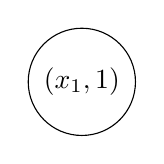
\begin{tikzpicture}[
    node distance=1.5cm and 2.5cm,
    mynode/.style={draw,circle,text width=1cm,align=center}
    ]

    \node[mynode] (1) {\((x_1,1)\)};
    \end{tikzpicture}
    \caption{$\mathcal{G}_1$ before unit propagation}
  \end{figure}

  Then we define $F_1' = F_0\{x_1\to 1\} =F_0\{x_1\to 1\} = F\{x_1 \to 1\}= \{(\neg x_2), (\neg x_3 \vee \neg x_4), (x_4 \vee x_2 \vee\neg x_3)\}$. We have an unit clause, therefore, we add a node$(x_2, 0)$, as this clause where associated in $F$ with the clause $(\neg x_1 \vee \neg x_2)$ we add an edge $(x_1,1)\to (x_2,0)$. As there were only a unit clause, we can define $F_1 = \{(\neg x_3 \vee \neg x_4), (x_4 \vee \neg x_3)\}$.\\
  
\begin{figure}[H]
  \centering
  \begin{tikzpicture}[
    node distance=1.5cm and 2.5cm,
    mynode/.style={draw,circle,text width=1cm,align=center}
    ]

    \node[mynode] (1) {\((x_1,1)\)};
    \node[mynode,right=of 1] (2) {\((x_2,0)\)};

    \draw[->] (1) -- (2) node[pos=0.1, sloped, above] {};

  \end{tikzpicture}
  \caption{$\mathcal{G}_1$ after unit propagation}
\end{figure}

Once we have $F_1$ and $\mathcal{G}_i$ we continue the iteration. Therefore we choose the variable $x_3$ (as $x_1$ and $x_2$ where already assigned) and assign it to $1$ as we initially decided. Therefore we define $\mathcal{G}_2 = \mathcal{G}_1 $, and immediately after we add the node $(x_3,1)$. We define $F_2' = \{(\neg x_4), (x_4)\}$. We have two unit clauses. Solving them as done above we have:

\begin{figure}[H]
  \centering
  \begin{tikzpicture}[
    node distance=1.5cm and 1.5cm,
    mynode/.style={draw,circle,text width=1cm,align=center}
    ]

    \node[mynode] (1) {\((x_1,1)\)};
    \node[mynode,right=of 1] (2) {\((x_2,0)\)};
    \node[mynode,below= of 2] (3) {\((x_3,1)\)};
    \node[mynode,right= of 3] (41) {\((x_4, 1)\)};
    \node[mynode,right= of 2] (40) {\((x_4, 0 )\)};
    \draw[->] (1) -- (2) node[pos=0.1, sloped, above] {};
    \draw[->] (3) -- (41) node[pos=0.1, sloped, above] {};
    \draw[->] (3) -- (40) node[pos=0.1, sloped, above] {};
    \draw[->] (2) -- (40) node[pos=0.1, sloped, above] {};
    \draw[->] (41) -- (40) node[pos=0.1, sloped, above] {};
    \draw[->] (40) -- (41) node[pos=0.5,  right] {Conflict};

  \end{tikzpicture}
  \caption{$\mathcal{G}_2$ after unit propagation}
\end{figure}

We can see that a conflict has arise. Therefore we can not continue iterating throw the process and $\mathcal{G}_{F,A} = \mathcal{G}_2$. Note that have we wanted to assign the values in other order, only a renaming would have been necessary. 
\end{example}
As we already stated, the purpose of the implication graph is to show the root of the conflict. That is, we want to know what assignments led to the conflict. This could be made by making a set of nodes $N=\{(x_j,a_j: j\in 1,...,k)\}$ such that every path from a decision node to the conflict has to include one node of the set. This will be named a cut, not confuse with the graph theory concept.\\


A conflict clause can be made from each cut $N$: once we have the set $N$, we can add a new clause $C = (l_1,...,l_k)$to $F$ such that $l_k = x_k$ if $a_k = 0$ and $l_k=\neg x_k$ otherwise.\\

Let's summarize what we know until know:
\begin{itemize}
\item[-] We know how to make implication graph.
\item[-] We know how to add conflict clauses from a cut of a implication graph with conflict.  
\end{itemize}

So we only has to learn strategies in order to detect cuts on implication graphs. Although every cut is enough to add conflict clauses, the most two common approaches are to choose cut are base on the idea of Unique Implication Point(UIP).  A UIP   is   a   vertex    that   dominates   both   vertices   corresponding   to   the   conflicting   variable. 

\begin{itemize}
\item Last UIP - choosing every decision node that has a path to the conflict.
\item First UIP - choosing the first unique point encountered. That is, following backward the implication graph from the conflict, choosing the first UIP.
\end{itemize}


The first UIP tend to produce smaller clauses and experimental results \cite{tichy2006clause} \cite{zhang2001efficient} provide proves in favor of it. It is commonplace on DPLL-based solver. The GRASP[\ref{sub:grasp}] algorithm was one of the first conflict driven solver, that is, a sat solver that implement a DPLL procedure based mainly on Clause Learning. 

\section{Other complete algorithms}

\subsection{Monien-Speckenmeyer (MS) Algorithm}
\label{alg:MS}
This algorithm is a variation of the DPLL-Shortest Clause algorithm, specifying that once you choose the shortest clause, all variables you choose should be from that clause until you satisfy it, as it will continue to be the shortest given that there is no clause with repeated literals as well as no clause that is a tautology. This algorithm (DPLLSC) on $k$-SAT generates a recursion such that $T(n) = \sum_{i=1}^kT(n-i)$. Under the hypothesis that MS does not has a under-exponential worst case complexity, then $T(n) = a^n$ for some $a \in (1,\infty)$.  Then

$$a^k = \sum_{i=1}^kT(i) = \frac{1-a^k}{1-a}$$

that solved in the equation $a^{k+1}+1 = 2a^k$. The difference between MS and DPLLSC is that MS includes an autark assignment search in addition to the unit clause search and generalizing the pure literal search (that would be a search of autarks of size 1). When we select a clause (the shortest) we first try to generate an autark with its variables and otherwise continue the algorithm.


\begin{algorithm}
  \caption{Monien-Speckenmeyer}\label{MS}
  \begin{algorithmic}[1]
    \Procedure{\texttt{MS}}{$F$}
    \If{$0 \in F$} \Return 0
    \EndIf
    \If{$F=1$} \Return 1
    \EndIf
    \State
    \If{$F$ contains a unit clause $\{p\}$} \Return $MS(F\{p\to 1\})$
    \EndIf
    \If{$F$ contains a pure literal l} \Return $MS(F\{l\to 1\}})$
  \EndIf
  \State Choose the shortest clause $C = \{u_1,...,u_m\}$
  \For{$i \in \{1,...,m\}$ }
  \State $\alpha_1 := \{u_1\to 0,...,u_{i-1}\to 0,u_i\to 1\}$
  \If{$\alpha_i$ is autark } \Return \texttt{MS}$(F\alpha_i)$
  \EndIf
  \EndFor
  \If{\texttt{MS}$(F\{u_1=1\})$} \Return 1
  \EndIf
  \State \Return $MS(F\{u_1=0\})$
\end{algorithmic}
\end{algorithm}


Other version of the algorithm repeats the last for-loop  in the successive calls of $F$ (calling \texttt{MS}$(F\alpha_i)$). Nonetheless we consider that with a deterministic heuristic (that, for example, choose the first clause between the set of clauses with minimum size) the result is equivalent and this provide a simpler algorithm.\\

For the $k$-SAT complexity analysis we have to consider whether or not an autark was found. If so, $T(n) \le T(n-1)$. Otherwise we are applying a non autark assignment that necessarily collide with a clause which size is at most $k-1$. Let us denote by $B(n)$ the number of recursive calls with n variables and under the hypothesis that there is a clause with at most $k-1$ variables. In this case $T(n) \le \sum_{i=1}^{k}B(n-i)$ and $B(n) \le \sum_{i=1}^{k-1}B(n-i)$. Both of these cases are worse than $T(n-1)$ so in order to study a worst case complexity we have to study the case when no autark is found. Under the hypothesis that $B(n) = a^n$ we get $a^k+1=2^{k-1}$. For $k=3$ we obtain $a=\frac{1 + \sqrt{5}}{2}$.



\subsection{Deterministic Local Search}

The local search procedure on sat context is the same as in other branches of computer science. The idea is that we start with an initial assignment $\alpha$ and search in the \emph{neighborhood} of $\alpha$ for a satisfying assignment, that is, those assignments that are close to $\alpha$ according to a distance $d$. 

\begin{definition}
  Let $\alpha$ and $\beta$ be assignments, we define the Hamming distance $d_\mathcal{H}$ as:
  $$d_\mathcal{H}(\alpha,\beta) = \left |\{ x \in Var(\alpha) \cup \Var(\beta)\}\right : \alpha(x) \ne \beta(x) \}\right |$$
  Note that in case that for every $y \in Var(\alpha) \backslash Var(\beta)$, we can  consider that $\alpha(y) = \upsilon$, and respectively with $\beta$.
\end{definition}

For every $\alpha$ we define its neighborhood as $D(\alpha,\delta) = \{\beta : d_\mathcal{H}(\alpha,\beta) \le \delta\}$. In order for this algorithm to work is necessary that $\delta > 0$ and is preferable that $\delta << |Var(\alpha) \cup Var(\beta)|$, in order to avoid doing a backtrack. The procedure determine whether or not there is a satisfying assignment for $F$ in $D(\alpha,\delta)$. The procedure take as input a CNF formula $F$, an assignment $\alpha$ and a positive integer $\delta$.

\begin{algorithm}
  \caption{Local Search\cite{schoning2013satisfiability}}\label{ds}
  \begin{algorithmic}[1]
    \Procedure{\texttt{LS}}{$F$, $\alpha$, $\delta$}
    \If{$F\alpha=1$} \Return Satisfiable
    \EndIf
    \If{$\delta=0$} \Return Unsatisfiable 
    \EndIf
    \State Choose $C={l_1,...,l_n}\inF$ such that $C\alpha=0$
  \For{$i \in \{1,...,n\}$ }
  \State \Return \texttt{LS}($F$, $\alpha\circ\{l_1 \to 1\}$, $\delta$ -1)
  \EndFor
\end{algorithmic}
\end{algorithm}


For 3-SAT the running time is $O(m3^\delta)$ where $m$ is the number of clauses. This technique is useful on formulas with a great density of satisfying assignments. Nonetheless, until now this is an incomplete algorithm. The strategy to prove incompleteness is the following. Let $F$ be a CNF formula, such that $Var(F)=\{x_1,...,x_n\}$ and consider $\delta = n//2+n\%2$ where // is the integer division and \% is the modulo, and $\alpha_a = \{x_1 \to a,...,x_n\to a\}$. Then by running \texttt{LS}($F,\alpha_0,\delta$) and \texttt{LS}($F,\alpha_1,\delta)$ we have a complete algorithm. The asymptotic complexity for this algorithm is $O(3^{n/2}) \approx O(2^{0.793n})$. Note that in this context we only work with two-valued assignment, as we are not dealing with partial assignments.\\

\begin{algorithm}
  \caption{Complete Local Search}\label{cls}
  \begin{algorithmic}[1]
    \Procedure{\texttt{CLS}}{$F$}
    \State $n \gets |Var(F)|$
    \State $\alpha_0 \gets \{x_i \to 0 : 1 \le i \le n\}$
    \State $\alpha_1 \gets \{x_i \to 1 : 1 \le i \le n\}$
    \State
    \If{\texttt{LS}($F$,$\alpha_0$, $n//2 + n\%2$)} \Return Satisfiable 
    \EndIf
    \State \Return \texttt{LS}($F$,$\alpha_1$, $n//2 + n\%2$)

\end{algorithmic}
\end{algorithm}



There is a natural way to generalize the idea of exploring all the space of assignments by coordinates local searches, and that is the covering codes.

\begin{definition}
  Let $X$ be a set of variables and let $A = \{\alpha_i: 1 \le i \le n\}$ a set of two valued assignments over $X$, and $\delta$ be a positive integer. The pair $(A,\delta)$ is a \emph{covering code with Hamming radius} $\delta$ if for any  two-valued assignment  $\alpha$  over $X$, there exists $\alpha'\in A$ such that $d_\mathcal{H} (\alpha, \alpha') < \delta$.
\end{definition}

We can note that the only important thing about $X$ on a covering code is the number of variables that it has. Therefore a covering code $(A,\delta)$ for $X=\{x_1,...,x_n\}$ is also, after a renaming, a covering code for $Y=\{y_1,...,y_n\}$, therefore we can consider that $A$ is a \emph{covering code of length} $n$. When no details about the set of variables is given other than its length $n$ we assume is a covering code over the set $X = \{x_1,...,x_n\}$


\begin{lemma}[lemma 5.3\cite{schoning2013satisfiability}]
For every $\epsilon > 0$ and $\delta \in (0, \frac{1}{2})$ there is a length $n_0$ so that there is a covering code $C_0 = (A=\{\alpha_i : 1\le i\le t\}, \delta n_0)$ of length $n_0$, with $t\le 2^{1-h(\delta)+\epsilon)n_0}$, where $h(\delta)$ is a  polynomial function on $\delta$.
\end{lemma}

\begin{proof}
  As done with the LLL, we will prove this result with probabilistic existence. We fix a set of variables $X=\{ x_i : 1 \le i \le n\}$ choose $t$ random assignments over $x$ following a uniform distribution. 

  We are going to prove that

  $$P(\exists \alpha_0 \forall i\in 1,...,t : d_\mathcal{H} (\alpha_0,\alpha_1)  > \delta n) < 1.$$

  We can see that 

\begin{equation}
\begin{split}
  P(\exists \alpha_0 \forall i\in 1,...,t : d_\mathcal{H} (\alpha_0,\alpha_1)  < \delta n)  & =  \sum_{\alpha_0\in A_{X} } \prod_{\alpha \in A} P(d_{\mathcal{H}} (\alpha_0,\alpha) > \delta n)\\
  & =  \sum_{\alpha_0\in A_{X} } \prod_{\alpha \in A} \left ( 1-P(d_{\mathcal{H}} (\alpha_0,\alpha) \le \delta n) \right )\\
  & =^{1.}  \sum_{\alpha_0\in A_{X} } \prod_{\alpha \in A} \left ( 1- \frac{\sum_{j=0}^{\delta n} {n\choose j}}{2^n} \right )\\
  & =^{2.}  2^n \left ( 1- \frac{\sum_{j=0}^{\delta n} {n\choose j}}{2^n} \right )^t\\
  & \le^{3.}  2^n  e^{-t \frac{\sum_{j=0}^{\delta n} {n\choose j}}{2^n}}\\
  & =^{4.}  \left (\frac{2}{e}\right )^n  \to_{n\to \infty} 0. 
\end{split}
\end{equation}

Where $A_{X}$ is the set of all two-valued assignments over $X$, 1. is because of results on binomials distribution, 2. is because the expresion is independent of eithet $\alpha_0$ and $\alpha$, 3. is because properties derived on the fact that $\lim (1-\frac{1}{n})^n \to e$ and 4. is because we have yet to define $t$ and we choose to define it as:
$$ t = \frac{n2^n}{\sum_{j=0}^{\delta n} {n\choose j}}.$$

As  $(\frac{2}{e}\right )^n  \to_{n\to \infty} 0 $ for some $n_0$ big enough we have that $P(\exists \alpha_0 \forall i\in 1,...,t : d_\mathcal{H} (\alpha_0,\alpha_1)  < \delta n) < 1$ and therefore there exists a covering on which  such $\alpha$ does not exists. To end the proof, we can also consider that 

$$ t = \frac{n_02^n_0}{\sum_{j=0}^{\delta n_0} {n_0\choose j}} \le 2^{1-h(\delta)+\epsilon)n_0} ,$$

for some polynomial function $h$ over $\delta$.

\end{proof}

\begin{remark}
  Every covering code $C = (\{\alpha_i : 1 \le i \l1 k\},\delta)$ of length $n$ can be \emph{truncated} to a covering code $C' = (\{\alpha_i' : 1 \le i \le k\},\delta)$ of length $m < n$  with $\alpha_i'$ defined as:
  $$
\alpha_i'(x)=
\begin{cases}
  \alpha_i(x) & x \in \{x_i:1\le i \le m\}\\
  \upsilon& \text{otherwise}.
\end{cases}
$$


\end{remark}

\begin{remark}
  Every covering code  $C = (\{\alpha_i : 1 \le i \l1 k\},\delta n_0)$ of length $n$ can be \emph{extended} to a covering code $C' = (\{\alpha_{i_1,...,i_{m//n+1}}' : 1 \le i_j \le k \},\delta n)$ of length $m > n$  with $\alpha_i'$ defined as:

  $$
\alpha_{i_1,...,i_{m//n+1}}'(x)=
\begin{cases}
  \alpha_{i_j}(x) & x \in \{x_i:n(j-1)+1\le i \le nj\}\\
  \upsilon& \text{otherwise}.
\end{cases}
$$

\end{remark}

Then, for every $\epsilon >0$, setting $\delta = 0.5$ we have a covering code $C_0$. We can suppose that for implementing our algorithm we have such covering without any need of processing for our algorithm, as we can brute-force look for it once, and then the algorithm can run as many time as required without any need of repeating those computations. 



\begin{algorithm}
  \caption{Covering Code Local Search}}\label{ccls}
\begin{algorithmic}[1]
  \State $C_0 \gets $ the covering code provided by the lemma for $\epsilon > 0\land \delta = 0.5$ 
  \Procedure{\texttt{Covering-Codes-LS}}{$F$}
  \State $n \gets |Var(F)|$
  \If{$n \le n_0$} \Return \texttt{CLS}($F$)
  \EndIf 
  \State $C=(A,\delta n_0) \gets $ the extended covering code of $C_0$ to $n$ variables
  \For{$\alpha \in A$ }
  \If{\texttt{LS}($F$, $\alpha$, $\delta n$) = Satisfiable} \Return Satisfiable
  \EndIf
  \EndFor
  \State \Return Unsatisfiable

\end{algorithmic}
\end{algorithm}

This algorithm for $3$-SAT run on $O((1.5 + \epsilon)^n)$\ref{dantsin2000deterministic}.\\


In fact what made this algorithm relevant is that its performs different from DPLL algorithm. No only on complexity but on what formulas it is able to solve efficiently.When we reduce a problem to SAT we have to take into account how a SAT will behave with our formulas, and from that we have to consider how to code it (if several alternative codings are available). LS allows us to not only design formulas that will work well in a DPLL search. For more information on how to take advantage of these differences see\ref{gomes2009exploiting}.
  
\subsection{GRASP - Todavía sin rehacer }
\label{sub:grasp}
We present now one of the most cited algorithms.  GRASP(Generic seaRch Algorithm for the Satisfiability Problem) was introduced by Marques-Silva and Sakallah\cite{marques1999grasp} that works on CNF formulas. It is based on clause learning techniques, and unit propagation. It divides the search process in four parts:

\begin{enumerate}
\item \texttt{Decide}: Chooses a decision assignment at each stage of the search process. Based of experimental results it uses the heuristic DLIS.
\item \texttt{Deduce}: Which implement a recursive unit propagation as done before.
\item \texttt{Diagnose}: Which implement a clause learning procedure.
\item \texttt{Erase}: Which delete assignments implied by the last decision.
\end{enumerate}


The method \texttt{Erase} is needed as the assignment is considered a global variable. The way that the algorithm work is that each time, either a new conflict clause is added to the formula, and therefore we \texttt{Erase} our last assignment to explore other options, or we find an assignment that satisfy the formula.



% \begin{algorithm}
%   \caption{GRASP}\label{bt}
%   \begin{algorithmic}[1]
%     \Procedure{\texttt{Search}($d$)}{$F$}
%     \State //d: decision level
%     \If{\texttt{Decide}($d$)} \Return 1
%     \EndIf
%     \While{True}
%     \If{\texttt{Deduce}(d) != Conflict}
%     \State \texttt{Search}(d+1)
%     \EndIf
%     \If{\texttt{Deduce}(d) == Conflict}
%     \If{\texttt{Diagnose}(d)}\texttt{ Erase(); } \Return Conflict
%     \EndIf
%     \EndIf
%     \State Erase
%     \EndWhile
%     \EndProcedure
%     \State \Return \texttt{Search}
% \end{algorithmic}
% \end{algorithm}

